\chapter{Monoidal Categories}
\marginnote{Thanks Jialu Bao for this lecture, and Shubh Agrawal for these scribe notes.}
\section{Categorifying Monoids}

We have been working thus far with typed PLs, specified using 
typing rules. We used categories to give them semantics and 
diagrams to depict the categories. We will now discuss PLs 
with resources, and use \emph{monoidal categories} to give 
them semantics, and use string diagrams to depict them.

First, let us recall the definition of monoid:


\begin{definition}[monoid]
    A triple $(M, \cdot, e)$ is a monoid if it satisfies:
    \begin{enumerate}
        \item \textbf{Associativity}: $\forall x, y, z \in M
            \,.\, (x \cdot y) \cdot z = x \cdot (y \cdot z)$
        \item \textbf{Identity}: $\forall x \in M \,.\,
            e \cdot x = x = x \cdot e$
    \end{enumerate}
\end{definition}

We have seen one way of categorifying monoids: construct a cateogry 
with one object and a morphism for each element of the monoid.
The monoid operation then corresponds to sequential composition 
and the monoid axioms correspond to the category axioms.

What if we instead categorify monoids by making the \emph{objects} form
a monoid and where the monoid operation corresponds to some notion
of parallel composition. Such categories are called 
\emph{monoidal categories}.
Monoidal categories are a category \(\mathcal{C}\) together with an
operation \(\otimes\), called the tensor product, and a distinguished
object \(I\). The axioms are then encoded as a certain relationship
between corresponding objects. Formally:

% For the axioms, we need a way to relate objects: 1.
% associativity:
% \((A \otimes B) \otimes C \leftright A \otimes (B \otimes C)\) 2.
% identity: \((I \otimes A) \leftright A \leftright (A \otimes I)\)

\begin{definition}[monoidal category]
    A category \(\mathcal{C}\) is a monoidal category if: 
    \begin{enumerate}
        \item there exists a bifunctor \(\otimes: 
            \mathcal{C} \times \mathcal{C} \to \mathcal{C}\)
        \item there exist natural isomorphisms:
            \begin{itemize}
                \item \( \alpha_{A, B, C} : A \otimes (B \otimes C) 
                    \Rightarrow (A \otimes B) \otimes C \)
                \item \( \lambda_{A} : I \otimes A \Rightarrow A \)
                \item \( \rho_A : A \Rightarrow A \otimes I \)
            \end{itemize}
        \item such that the following diagrams commute:
    \end{enumerate}
    \begin{tikzcd}[column sep=large, row sep=large]
    ((A \otimes B) \otimes C) \otimes D 
      \arrow[r, "\alpha_{A,B,C} \otimes \text{id}_D"] 
      \arrow[d, "\alpha_{A \otimes B,C,D}"'] 
      & (A \otimes (B \otimes C)) \otimes D 
        \arrow[r, "\alpha_{A,B \otimes C,D}"] 
      & A \otimes ((B \otimes C) \otimes D) 
        \arrow[d, "\text{id}_A \otimes \alpha_{B,C,D}"] \\
    (A \otimes B) \otimes (C \otimes D) 
      \arrow[rr, "\alpha_{A,B,C \otimes D}"'] 
      & & A \otimes (B \otimes (C \otimes D))
    \end{tikzcd}

    \begin{tikzcd}[column sep=huge]
    (A \otimes I) \otimes B 
      \arrow[rr, "\alpha_{A,I,B}"] 
      \arrow[dr, "\rho_A \otimes \text{id}_B"'] 
      & & A \otimes (I \otimes B) 
        \arrow[dl, "\text{id}_A \otimes \lambda_B"] \\
      & A \otimes B &
    \end{tikzcd}
\end{definition}

The conditions that these diagrams commute are often simply referred 
to as ``coherence conditions.'' The intuition is that the 
three natural isomorphisms need to 
interact with each other well in the sense that if we take any 
two paths between objects, then they are equivalent. 
Proving those two diagrams commute is sufficient to prove the 
\emph{coherence theorem}, which makes the notion described 
above precise.

Let us define some of the other terms in the definition:

\begin{definition}[bifunctor]
A functor from the product category \(\mathcal{C} \times \mathcal{C}\) 
to \(\mathcal{C}\).
\end{definition}

\begin{definition}[natural isomorphism]
natural isomorphism: a natural transformation \(\eta : F \Rightarrow G\)
is a natural isomorphism if for every object \(X \in \mathcal{C}\), the
component \(\eta_X\) is an isomorphism. More concretely, we have the
following diagram for every $f : X \to Y$ in $\mathcal{C}$:

\begin{tikzcd}[column sep=large, row sep=large]
F(X) 
  \arrow[r, bend left=30, "\eta_X"] 
  \arrow[d, "F(f)"'] 
  & G(X) 
    \arrow[l, bend left=30, "\eta_X^{-1}"] 
    \arrow[d, "G(f)"] \\
F(Y) 
  \arrow[r, bend left=30, "\eta_Y"'] 
  & G(Y) 
    \arrow[l, bend left=30, "\eta_Y^{-1}"]
\end{tikzcd}
\end{definition}

With these in hand, we can now define how to turn a monoid
\((M, \cdot, e)\) into a monoidal category:
\begin{itemize}
    \item The objects are the elements of $M$
    \item Morphisms are only the identity morphism on each object
    \item The tensor product $a \otimes b$ is the monoid operation 
        $a \cdot b$
    \item The tensor product on morphisms $f \otimes g$ is trivial
        because both $f$ and $g$ are identity morphisms; thus, we
        have $\text{id}_A \otimes \text{id}_B = \id_{A \otimes B}$.
    \item We must show that the \(\otimes\) defines a functor. It clearly
        respects identity by the definition above. showing it respects
        composition amounts to proving the following:
        \((f_1 \otimes f_2) \circ (g_1 \otimes g_2) 
        =  f_1 \circ g_1 \otimes f_2 \circ g_2\).
        This holds because all morphisms are the identity 
    \item The objects we need to define natural transformations between are
        exactly equal by the monoid axioms, so we just define the transformations 
        to be the identity on each component.
\end{itemize}

\section{String Diagrams}

In string diagrams, we represent objects with wires and morphisms with
boxes (including an identity). Sequential compositions correspond to
wiring boxes together. Tensor product for objects corresponds to
juxataposing wires next to each other, and tensor products of wires is
putting boxes next to each other. The monoid unit corresponds to a
``phantom wire'' which need not be drawn.

\begin{center}
  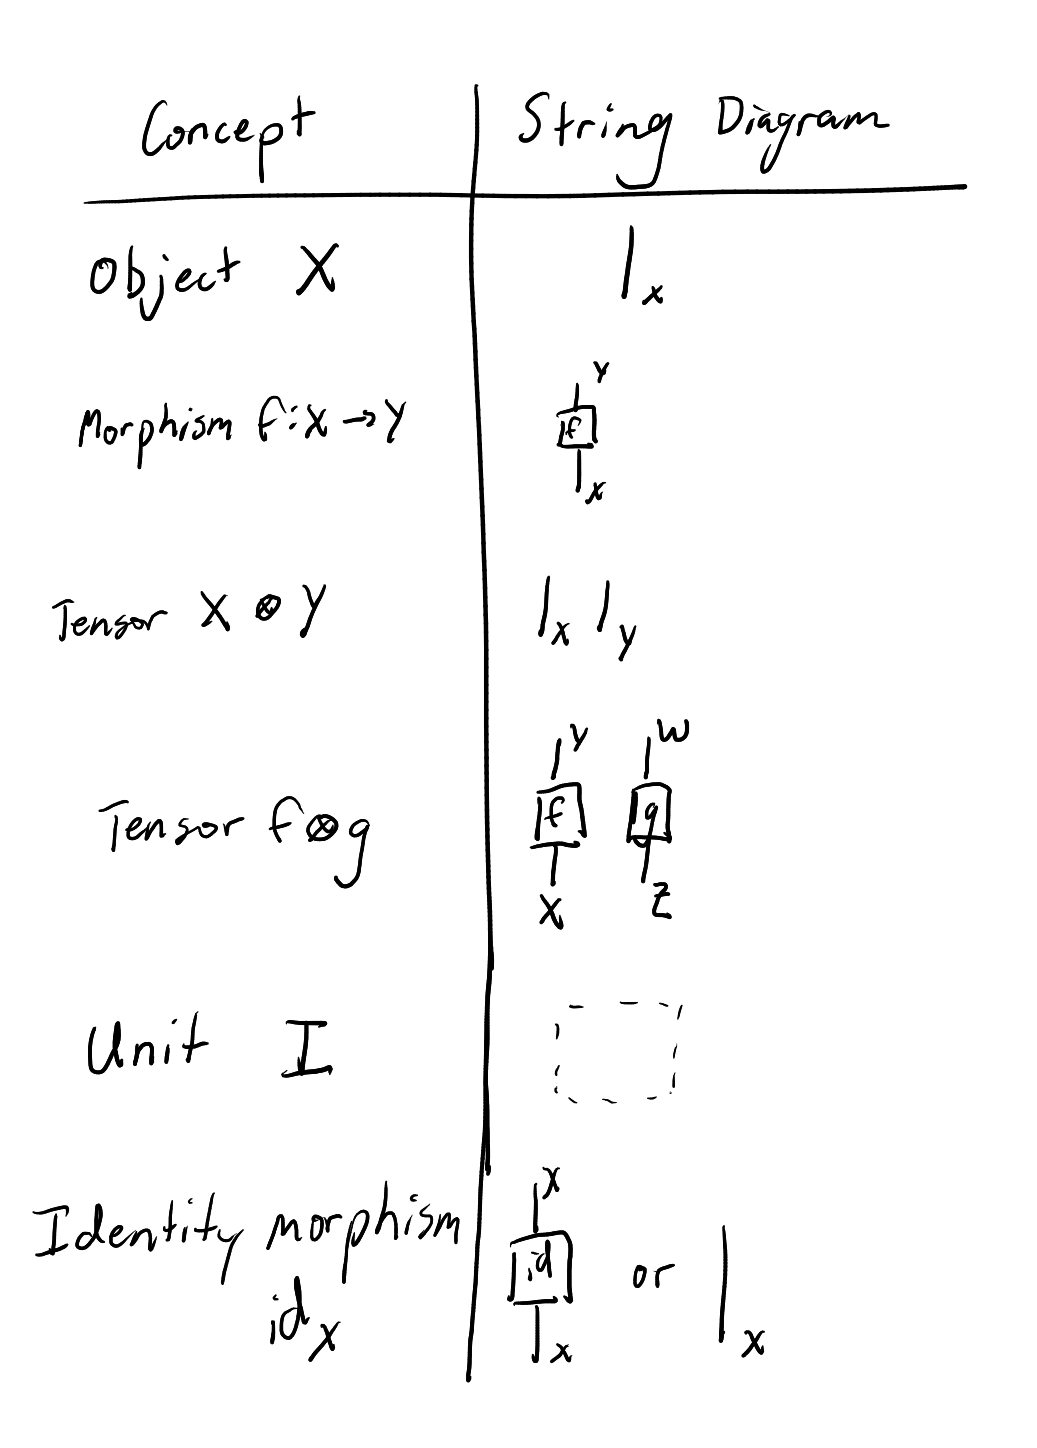
\includegraphics[width=250px]{fig/monoidal-categories-concepts.png}
\end{center}
Many of the laws correspond to extremely intuitive facts about diagrams:

\begin{center}
  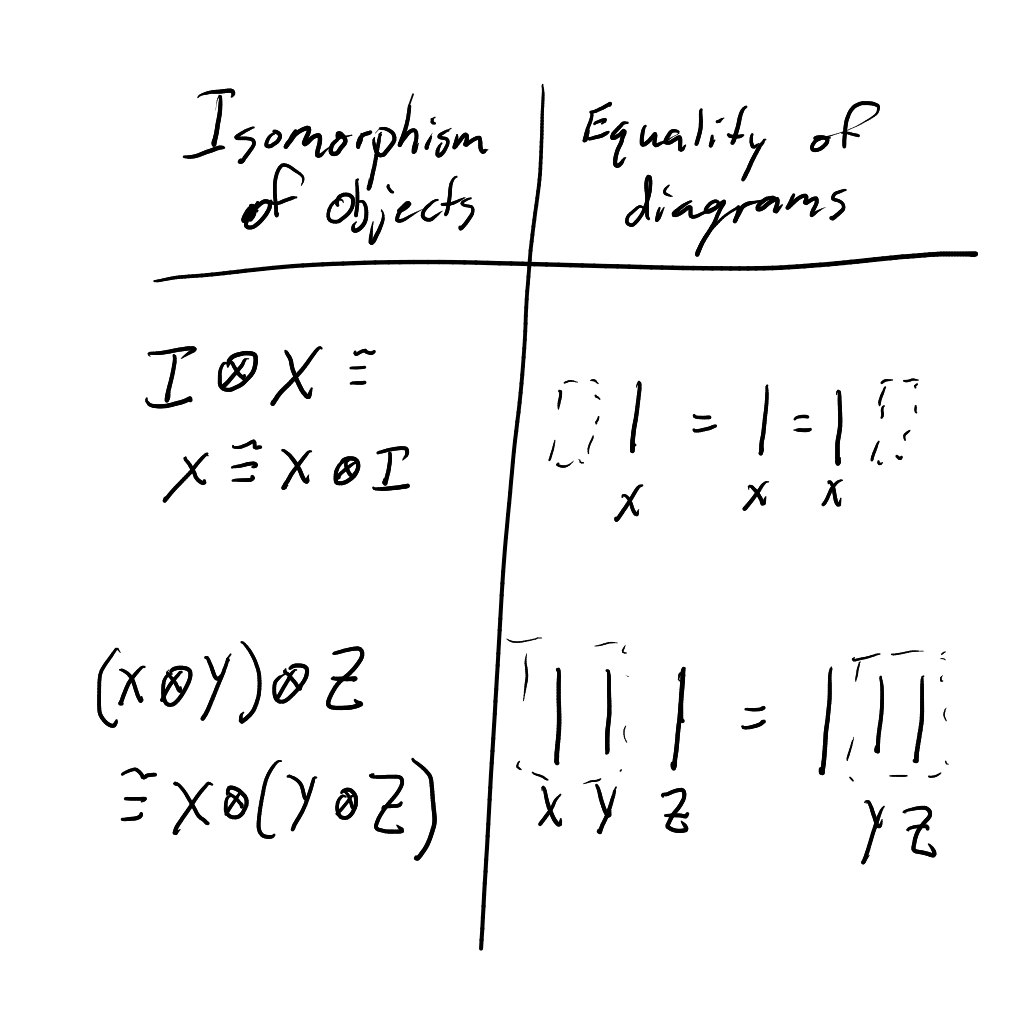
\includegraphics[width=250px]{fig/monoidal-categories-isos.png}
  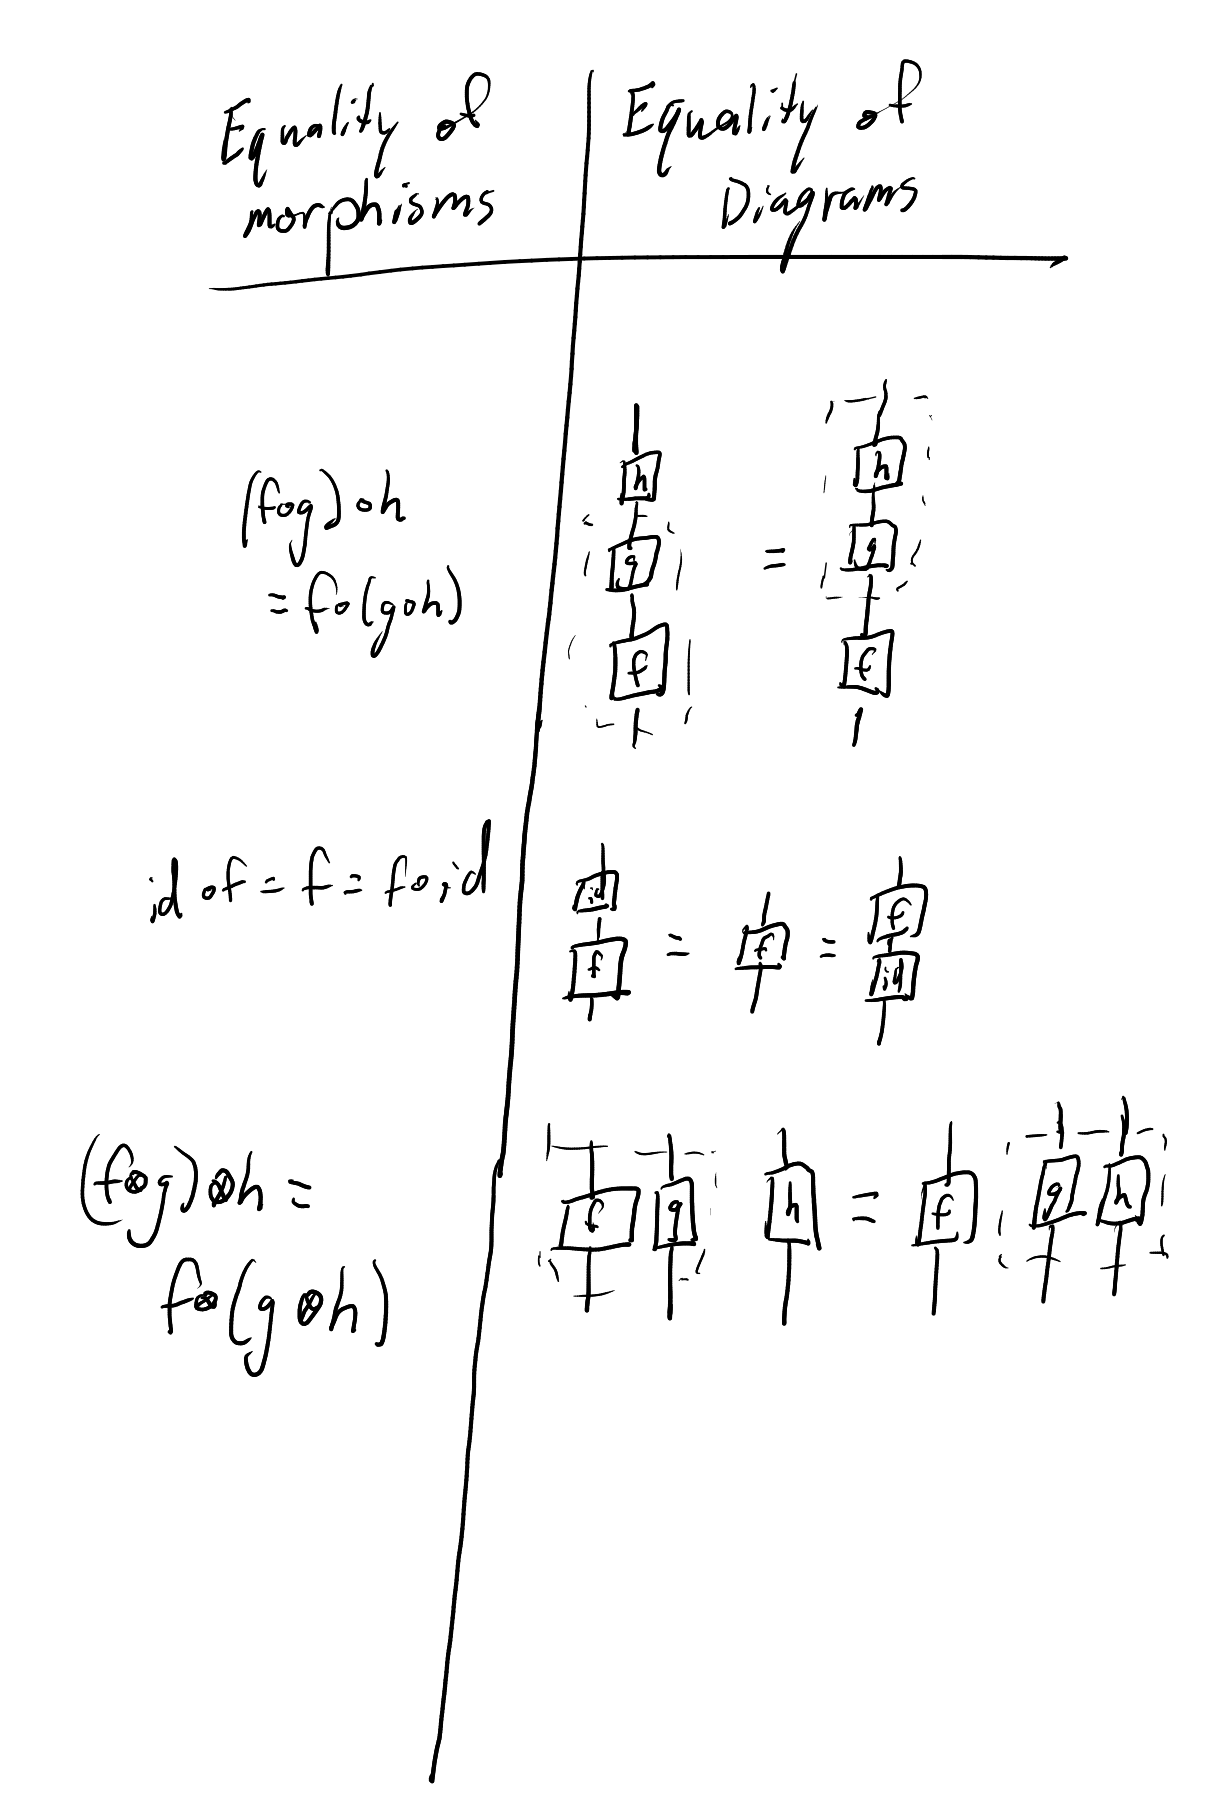
\includegraphics[width=250px]{fig/monoidal-categories-morphisms.png}
\end{center}

In any monoidal category, we have a notion of ``generating objects and
morphisms,'' which can't be decomposed into the tensor product of other
objects; the category is then formed by taking all the possible tensor
products.

\section{Example: Real Numbers}

Consider the preorder of real numbers viewed as a category. We can
define the tensor product on objects to be addition and the monoidal
unit to be 0. Given two morphisms \(n_1 \to n_2\), \(m_1 \to m_2\), the
tensor product is the morphism \(n_1 + m_1 \to n_2 + m_2\), which we
know exists by monotonicity of addition. Similar to the monoid example,
the natural isomorphisms are the identity on each component because the
corresponding objects are equal.

We can also use string diagrams to prove facts about this
preorder. Here, we have diagrams representing proofs of \(v+x \le y\),
\(w + u \le x + z\), \(t \le v + w\). We can then wire the boxes
together to get a proof of \(t + u \le y + z\): 

\begin{center}
  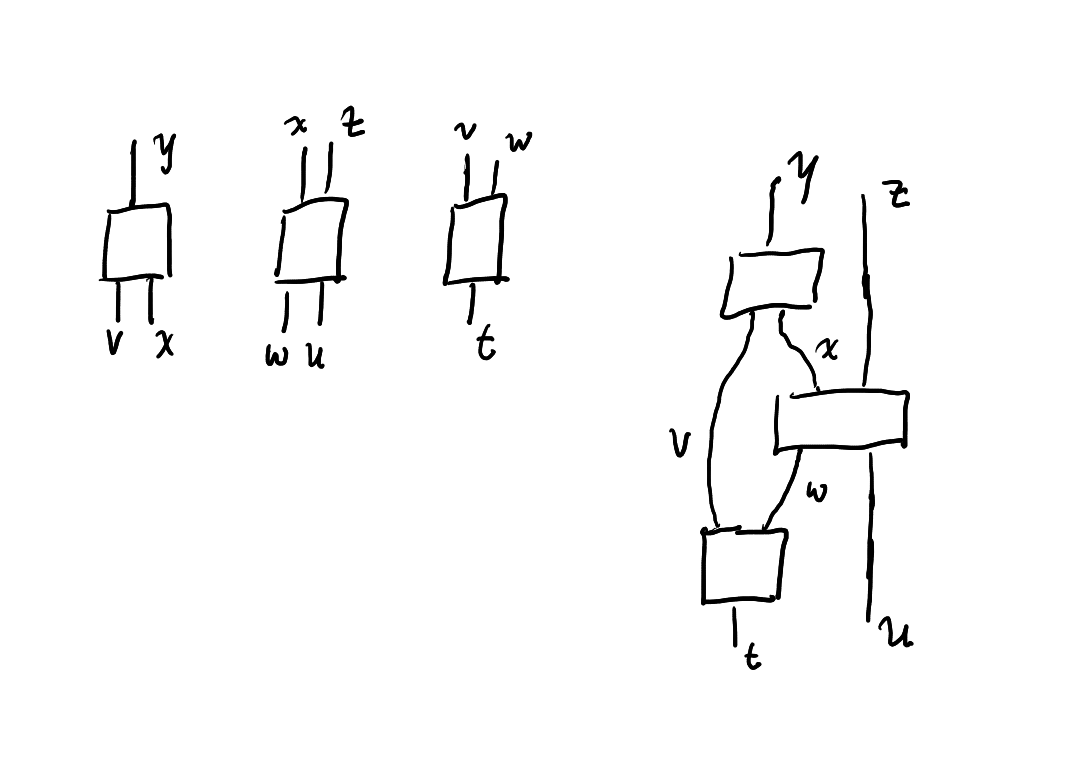
\includegraphics[width=250px]{fig/monoidal-categories-reals.png}
\end{center}


\section{Example: Cartesian Categories}

If \(\mathcal{C}\) has a product \(\times\) and terminal object \(T\),
then this forms a monoidal category with \(\otimes = \times\) and
\(I = T\).

The natural isomorphism for associativity was proven in Homework 1:
\(\alpha = \langle \langle \pi_1, \pi_1 \circ \pi_2 \rangle, 
\pi_2 \circ \pi_2 \rangle\).
We also have \(\lambda = \pi_1\) and
\(\rho = \langle \star, \text{id}_A \rangle\).

In the typed PL perspective, we had rules for operating with products
and the terminal object. We could then use these to construct more
complicated terms. For example, we might ask given terms \(x : A \vdash M : B\) 
and \(\langle x, y \rangle : A \times B \vdash N : C\), how can we construct
a term \(T\) such that \(x : A \vdash T : C\)? We can do this with our
term language. We can also do it in string diagrams: 

\begin{center}
  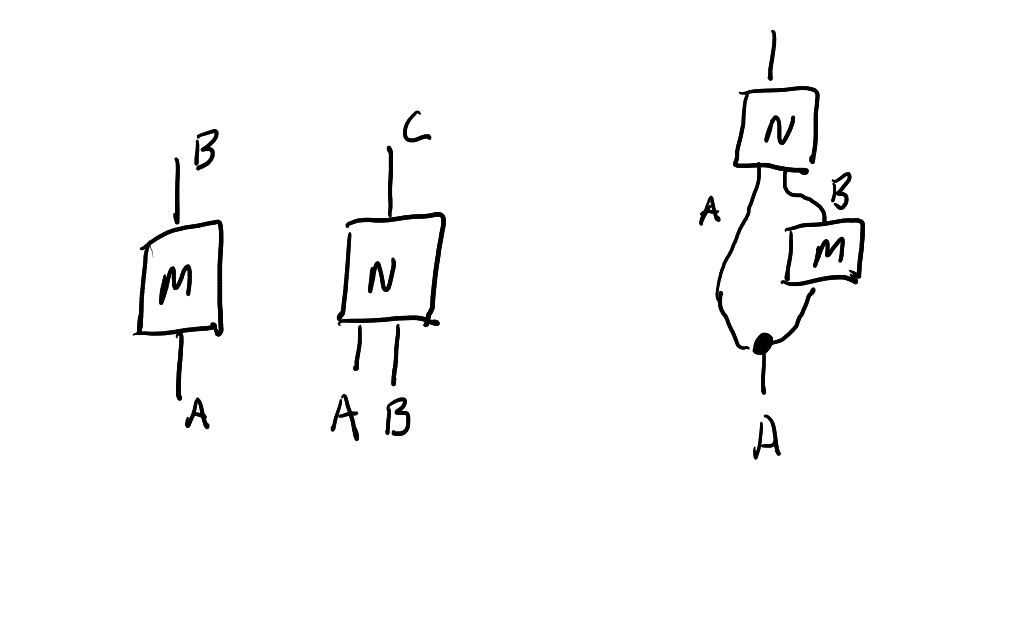
\includegraphics[width=250px]{fig/monoidal-categories-ccc.png}
\end{center}


Doing this requires a \emph{copy} operation, which allows us to duplicate \(A\).


\section{Additional Structure}

\subsection{Symmetry}

Notice that in both examples given, we have that the tensor product is
commutative. The categories where this holds are called \emph{symmetric
monoidal categories}, which come equipped with an additional natural
transformation \(\gamma : A \otimes B \Rightarrow B \otimes A\). We get
the following laws: 

\begin{center}
  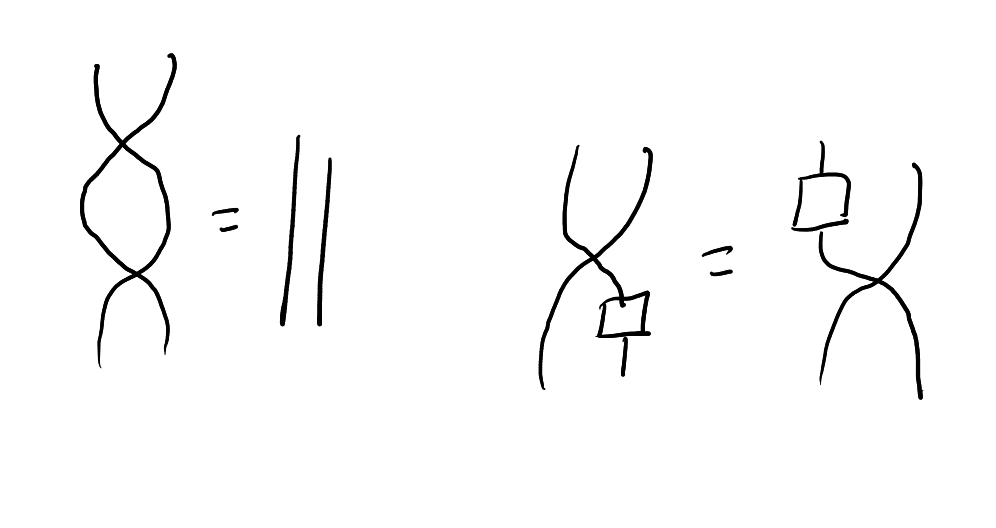
\includegraphics[width=250px]{fig/monoidal-categories-sym.png}
\end{center}


\subsection{Copy and Discard}

In order to encode all the same operations we expected in our STLC
with pairs and unit, we needed a copy operation. The copy operation
is a morphism $A \to A \otimes A$ for each $A$.
In general, monoidal categories won't always have a copy operation. This
corresponds to the intuition of monoidal categories as representing
resources -- if our resource can be copied, then our category would have
a copier. If not, then it wouldn't.

Often, when we have a copy operation, we also have a discard operation 
$A \to I$. These operations will satisfy the following rules: 

\begin{center}
  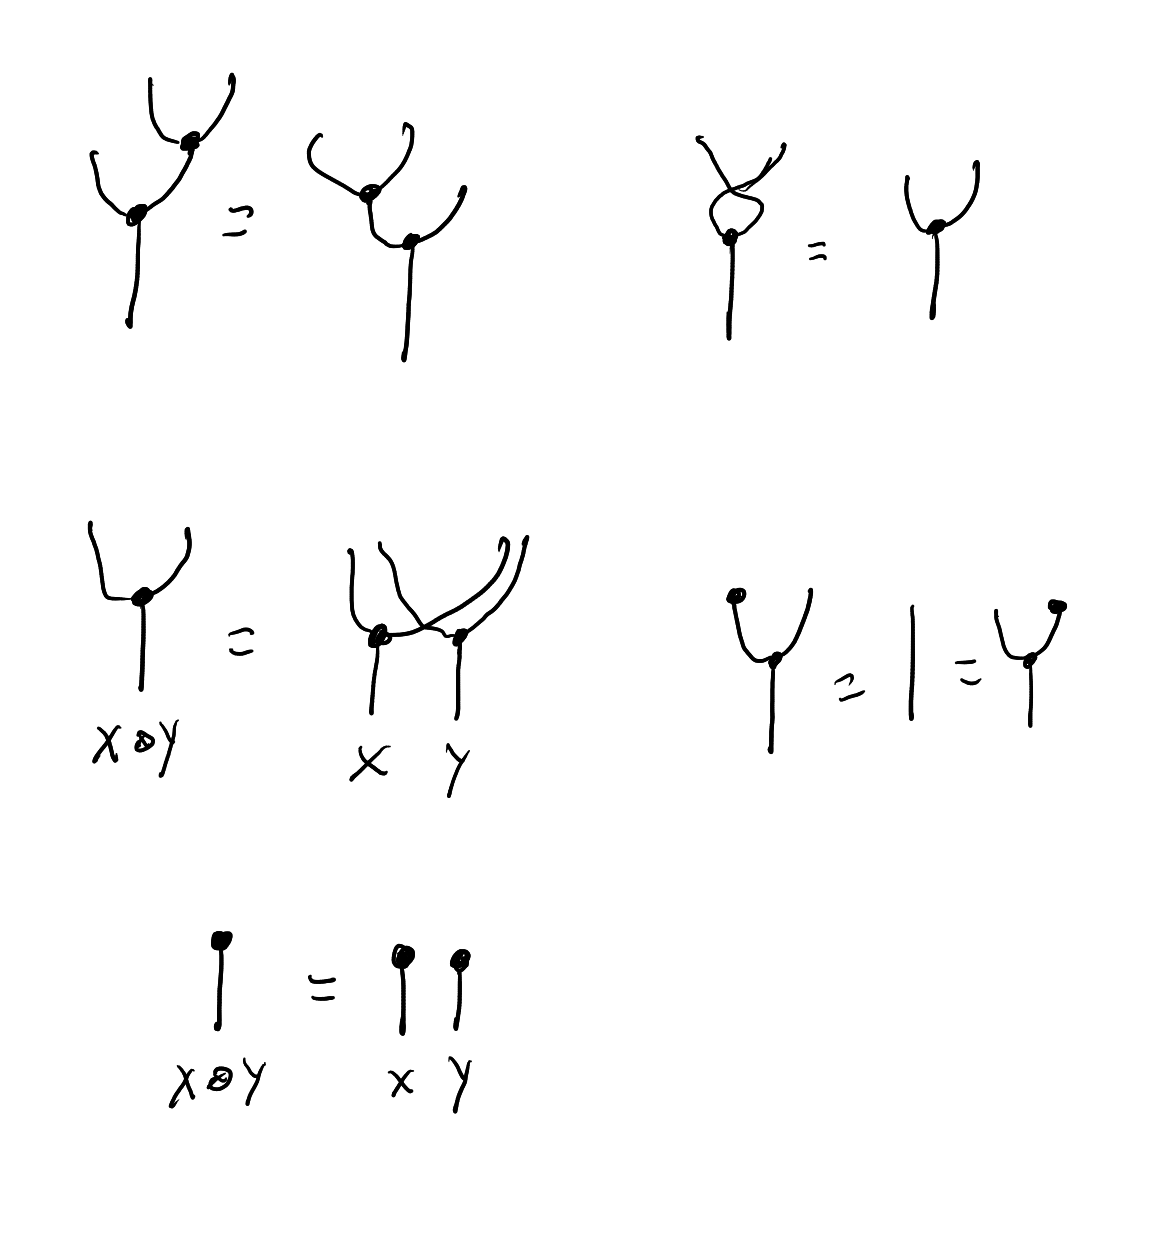
\includegraphics[width=250px]{fig/monoidal-categories-cd.png}
\end{center}

